\section{Erdbeschleunigung mit dem Pendel}


\subsection{Versuchsbeschreibung}

In diesem Experiment wird die Schwingung eines physikalischen Pendels untersucht, um die Erdbeschleunigung $g$ zu bestimmen. Die Schwingungsgleichung für das physikalische Pendel lautet
$$J \ddot \varphi = - mgl_s \sin(\varphi)\text{.}$$
Dabei ist $J$ das Gesamtträgheitsmoment des Pendels und $l_s$ der Abstand vom Aufhängepunkt zum Schwerpunkt des Pendels, sowie $\varphi$ der Auslenkwinkel aus der Ruhelage. Auf der rechten Seite der Gleichung steht das rücktreibende Drehmoment, welches durch die Gravitationskraft hervorgerufen wird. Für kleine Winkel, bei denen $\sin(\varphi) \approx \varphi$ näherungsweise gilt, ergibt sich die lineare, homogene Differentialgleichung zweiter Ordnung
$$\ddot \varphi = -\frac{mgl_s}J \varphi\text{.}$$
Diese Gleichung hat die allgemeine Lösung
$$\varphi(t) = A\cdot \cos(\omega t)+ B\cdot \sin(\omega t)\text{.}$$
Die Kreisfrequenz $\omega$ dieser Schwingung ist gegeben durch
$$\omega^2 = \frac{mgl_s}J\text{.}$$
Da das Trägheitsmoment $J$ des Pendels schwierig zu bestimmen ist, umgehen wir dieses Problem. Das betrachtete Pendel besteht aus einem Winkelaufnehmer-Profil, der Pendelstange und einem zylindrischen Pendelkörper.

\begin{figure}[h]
	\centering
	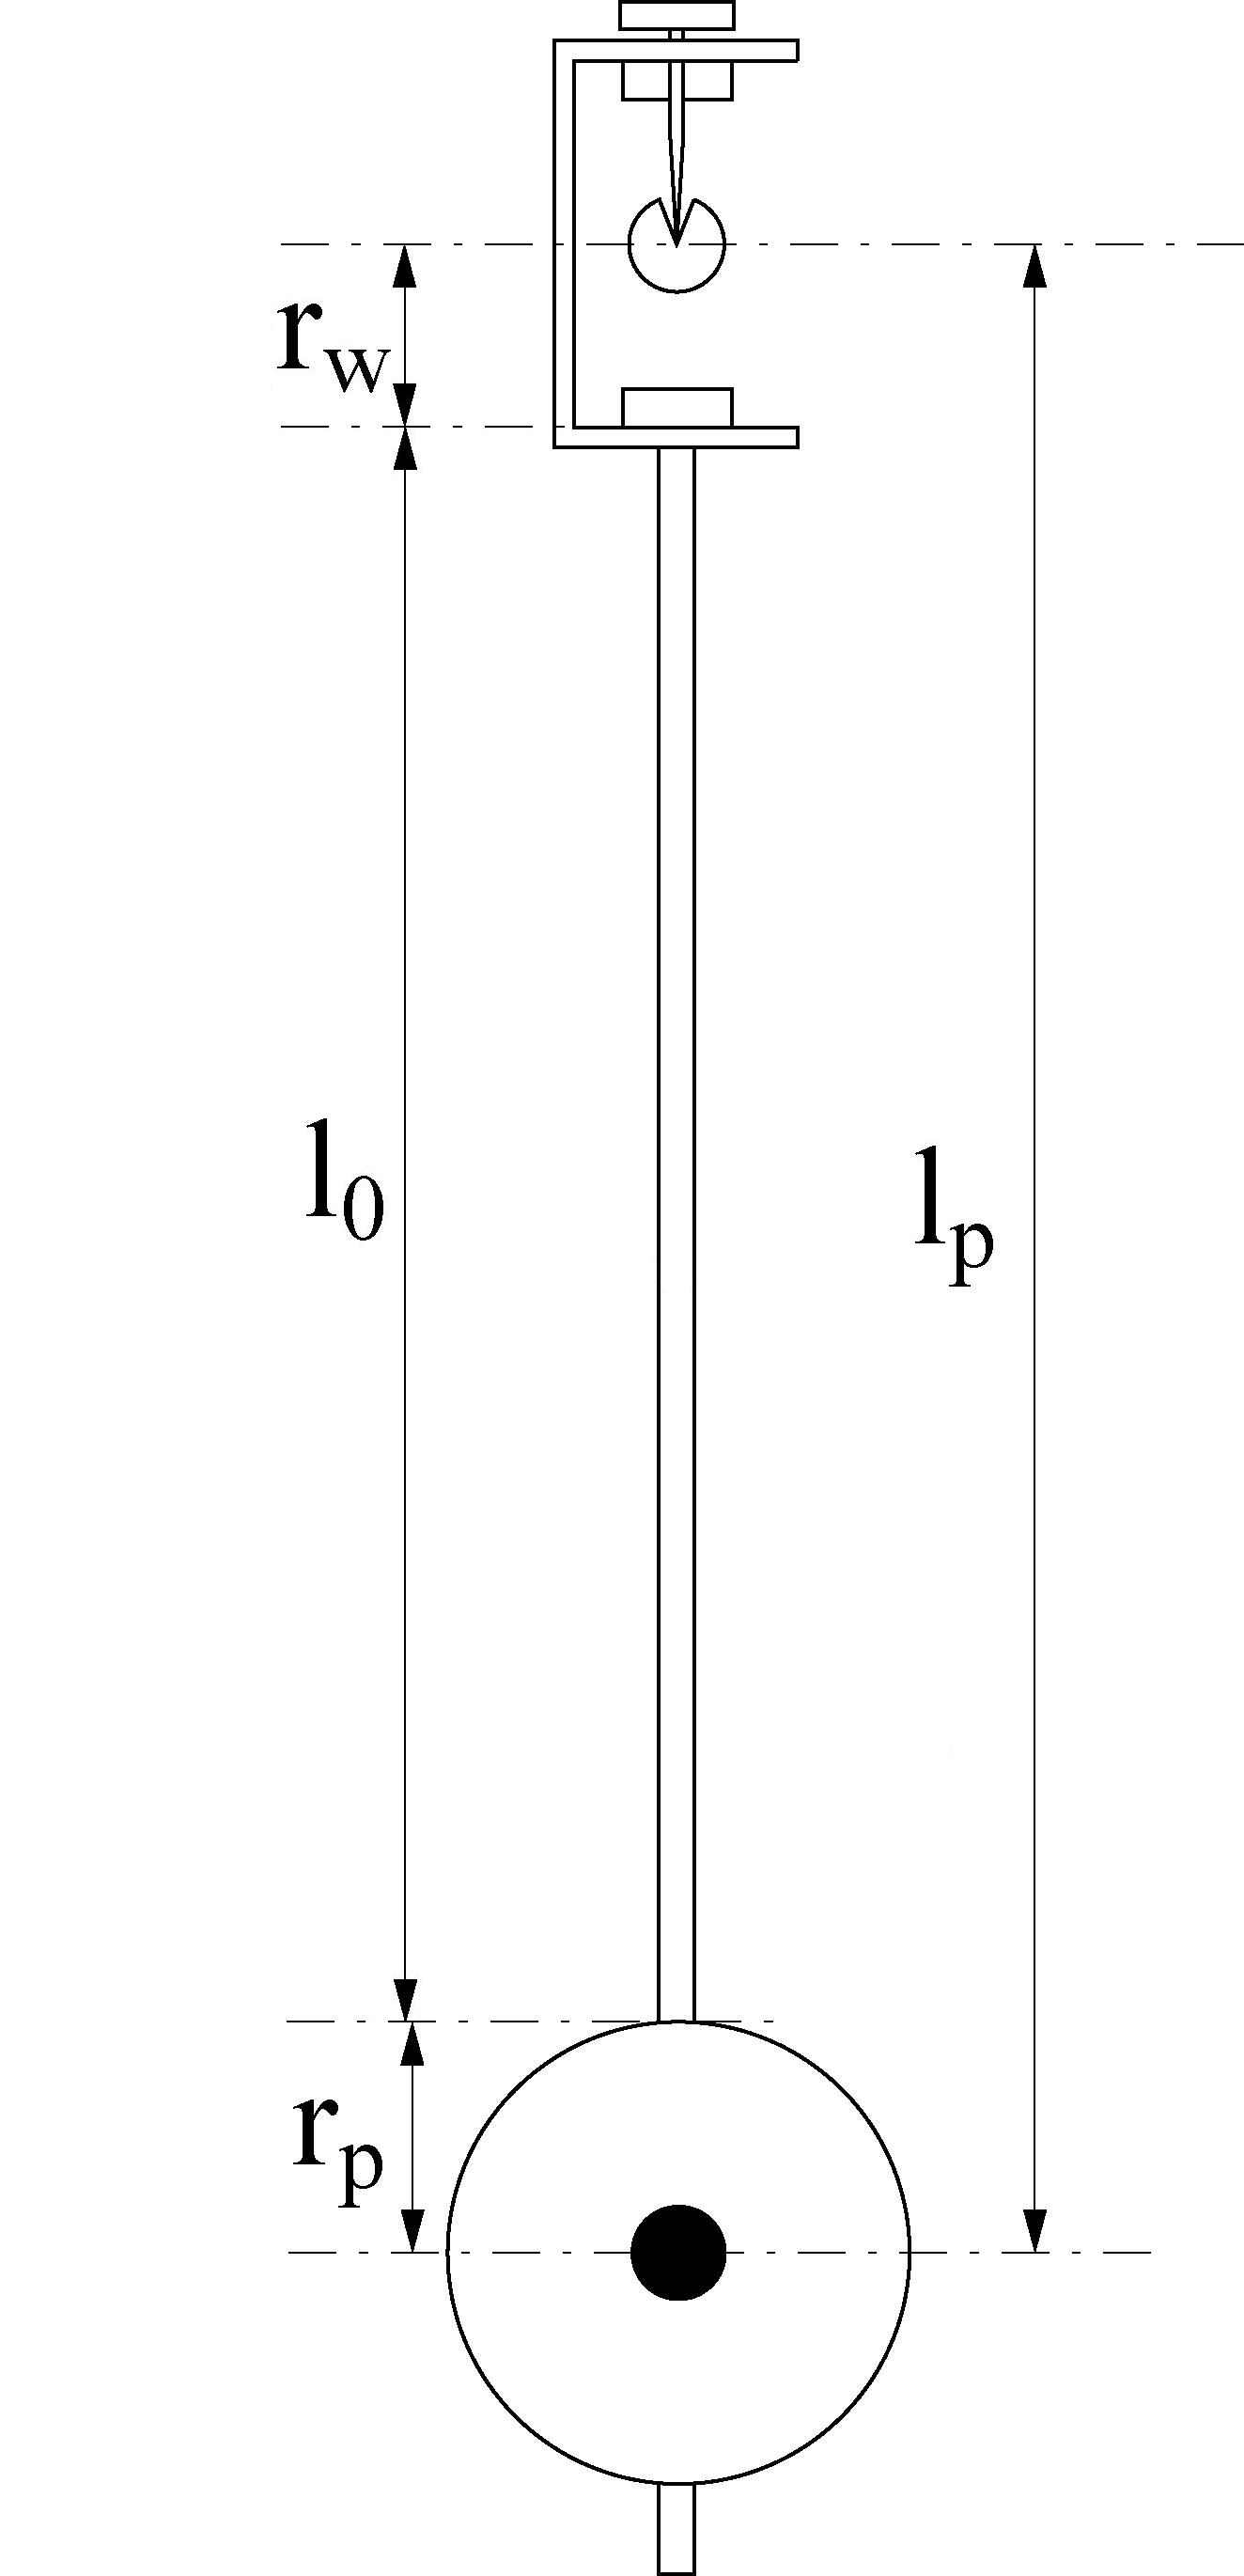
\includegraphics[scale=0.15]{bilder/Pendel_Zeichnung_be.jpg}
	\caption{Schematische Zeichung des Pendels}
\end{figure}

Wir bestimmen zunächst die Schwingungsfrequenz $\omega_{st}$ der Stange. Anschließend wird der Pendelkörper so an der Stange angebracht, dass das Pendel mit Pendelkörper und Stange die gleiche Schwingungsfrequenz hat wie die Stange allein. Sind $D_{st}$ und $D_p$ die maximalen Rückstellmomente von Stange und Pendelkörper und $J_{st}$ und $J_p$ die entsprechenden Trägheitsmomente, so gilt für die Schwingungfrequenz der Stange allein
$$\omega_{st}^2 = \frac{D_{st}}{J_{st}}\text{.}$$
Für den Pendelkörper allein gilt analog
$$\omega_p^2 = \frac{D_p}{J_p}\text{.}$$
Da die Rückstellmomente und die Trägheitsmomente additiv sind, ergibt sich die Frequenz des physikalischen Pendels mit Stange und Pendelkörper zu
$$\omega^2 = \frac{D_{st} + D_p}{J_{st} + J_p} = \omega_{st}^2 \frac{1+\frac{D_p}{D_{st}}}{1+\frac{J_p}{J_{st}}}\text{.}$$
Ist der Pendelkörper nun so eingestellt, dass $\omega = \omega_{st}$, so muss $\frac{D_p}{D_{st}} = \frac{J_p}{J_{st}}$ gelten. Daraus erhält man schließlich
$$\omega_p = \omega_{st} = \omega\text{.}$$
Das Pendel lässt sich so betrachten als bestünde es nur aus dem Pendelkörper. Mit dem Trägheitsmoment des geometrisch einfachen Pendelkörpers und dem Satz von Steiner ergibt sich
$$J_p = \frac 12 m_p r_p^2 + m_pl_p^2\text{.}$$
Damit lässt sich nun die Kreisfrequenz des Pendels ausdrücken
$$\omega^2 = \omega_p^2 = \frac{D_p}{J_p} = \frac{m_pgl_p}{\frac 12 m_pr_p^2+m_pl_p^2}\text{.}$$
Durch Umformen folgt schließlich die Formel für die Erdbeschleunigung
$$g = \omega^2l_p \left( 1 + \frac 12 \frac{r_p^2}{l_p^2} \right)\text{.}$$
Durch Messung des Radius $r_p$ und der Länge $l_p$, sowie der Periodendauer $T = \frac{2\pi}{\omega}$, lässt sich somit die Erdbeschleunigung bestimmen.

\subsection{Versuchsaufbau und -durchführung}


\subsection{Auswertung}
Nach der Kalibrierung der Winkelgeschwindigkeit wurden folgende Längen für das Pendel mit Pendelkörper gemessen:

\begin{table}[H]
\centering
\begin{tabular}{c|c|c}
$r_w$ & $l_0$ & $r_p$ \\
\hline
$2.535\text{cm} \pm 0.005\text{cm}$ & $61.5\text{cm}\pm 0.069\text{cm}$ & $3.998\text{cm} \pm 0.003\text{cm}$
\end{tabular}
\caption{Ergebnisse der Längenmessungen}
\end{table}

Das ergibt eine Pendellänge $l_p = r_w + l_0 + r_p = 68.033 \text{cm}$ mit einem Fehler von $\sigma_{l_p} = 0.07 \text{cm}$. Aus den mit dem Sensor-Cassy aufgenommenen Rohdaten ergeben sich folgende Zeitpunkte an denen das Pendel mit bzw. ohne Pendelkörper die $n$-te maximale Auslenkung annimmt:

\begin{table}[H]
\centering

\begin{adjustbox}{width=\textwidth}
\begin{tabular}{c|cccccccccc}
Schwingung & 1 & 10 & 20 & 30 & 40 & 50 & 60 & 70 & 80 & 90 \\
\hline
Zeitpunkt (Pendelkörper) [s] & 0.48 & 15.38 & 31.94 & 48.48 & 65.04 & 81.56 & 98.11 & 114.68 & 131.28 & 147.84 \\
Zeitpunkt (nur Stange) [s] & 1.5 & 16.44 & 33.01 & 49.59 & 66.14 & 82.73 & 99.32 & 115.86 & 132.46 & 149.05
\end{tabular}
\end{adjustbox}
\end{table}

\begin{table}[H]
\centering
\begin{adjustbox}{width=\textwidth}
\begin{tabular}{c|cccccccccc}
Schwingung & 100 & 110 & 120 & 130 & 140 & 150 & 160 & 170 & 180 & 190 \\
\hline
Zeitpunkt (Pendelkörper) [s] & 164.36 & 180.9 & 197.46 & 214.02 & 230.56 & 247.12 & 263.68 & 280.22 & 296.8 & 313.34 \\
Zeitpunkt (nur Stange) [s] & 165.64 & 182.18 & 198.8 & 215.34 & 231.92 & 248.47 & 265.08 & 281.62 & 298.23 & 314.83
\end{tabular}
\end{adjustbox}
\end{table}

\begin{figure}[h]
	\centering
	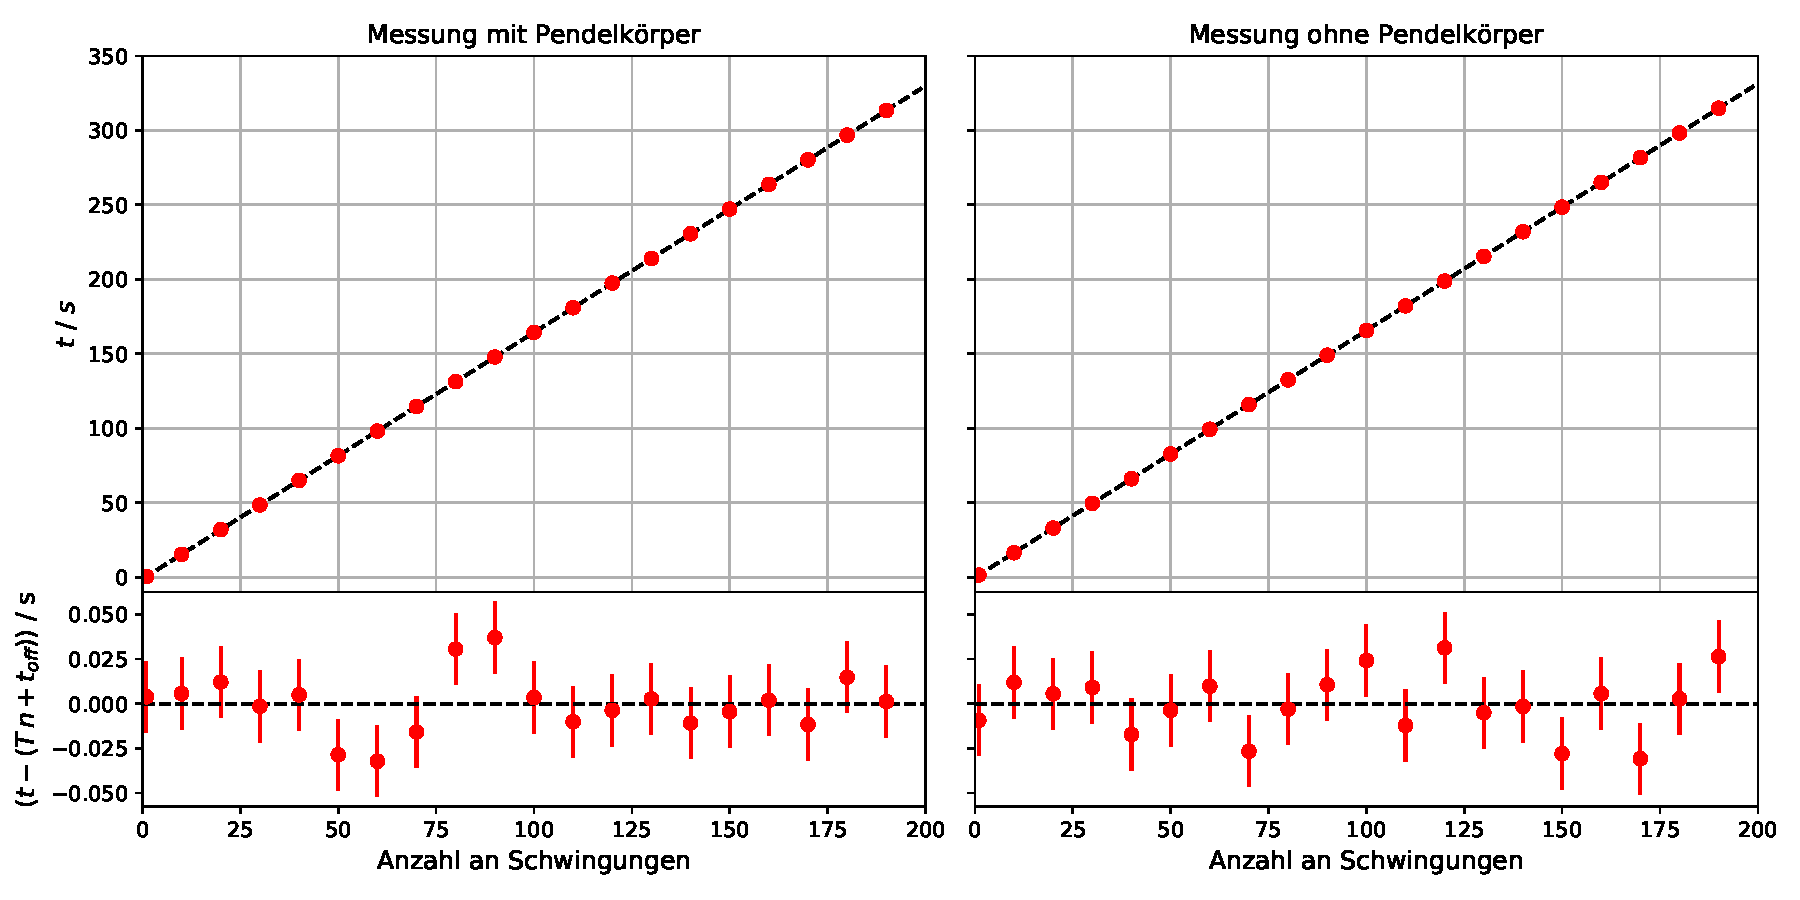
\includegraphics[width = \textwidth]{plots/regression.pdf}
	\caption{Regression und Residuenplot für Datenpunkte aus dem Versuch mit und ohne Pendelkörper}\label{plot:regression}
\end{figure}

Diese Datenpunkte wurden mit einer Genauigkeit von $\sigma_{t} = 0.02\text{s}$ bestimmt. Eine lineare Regression der Zeitpunkte mit Residuenplot ist in Abbildung \ref{plot:regression} zu sehen und liefert eine Periodendauer von $T_p = 1.65536 \text{s} \pm 7\cdot 10^{-5} \text{s}$ ($\chi^2 = 0.73$) bzw. $T_{st} = 1.65764 \text{s} \pm 7\cdot 10^{-5}\text{s}$ ($\chi^2 = 0.80$). Die $\chi^2$-Werte sind dabei zufriedenstellend. Mit $\omega = \frac{2\pi}{T}$ führt das zu den Kreisfrequenzen $\omega_p = 3.79566\, \text{Hz}\, \pm 0.00018\, \text{Hz}$ und $\omega_{st} = 3.79043\, \text{Hz} \,\pm 0.00018\, \text{Hz}$. Dabei ist der Fehler in $\omega$ nach Gaußscher Fehlerfortpflanzung durch
$$ \sigma_\omega = \left| \frac{\partial \omega (T)}{\partial T} \sigma_T \right | = \frac{2\pi}{T^2} \sigma_T $$
gegeben.

\begin{figure}[h]
	\centering
	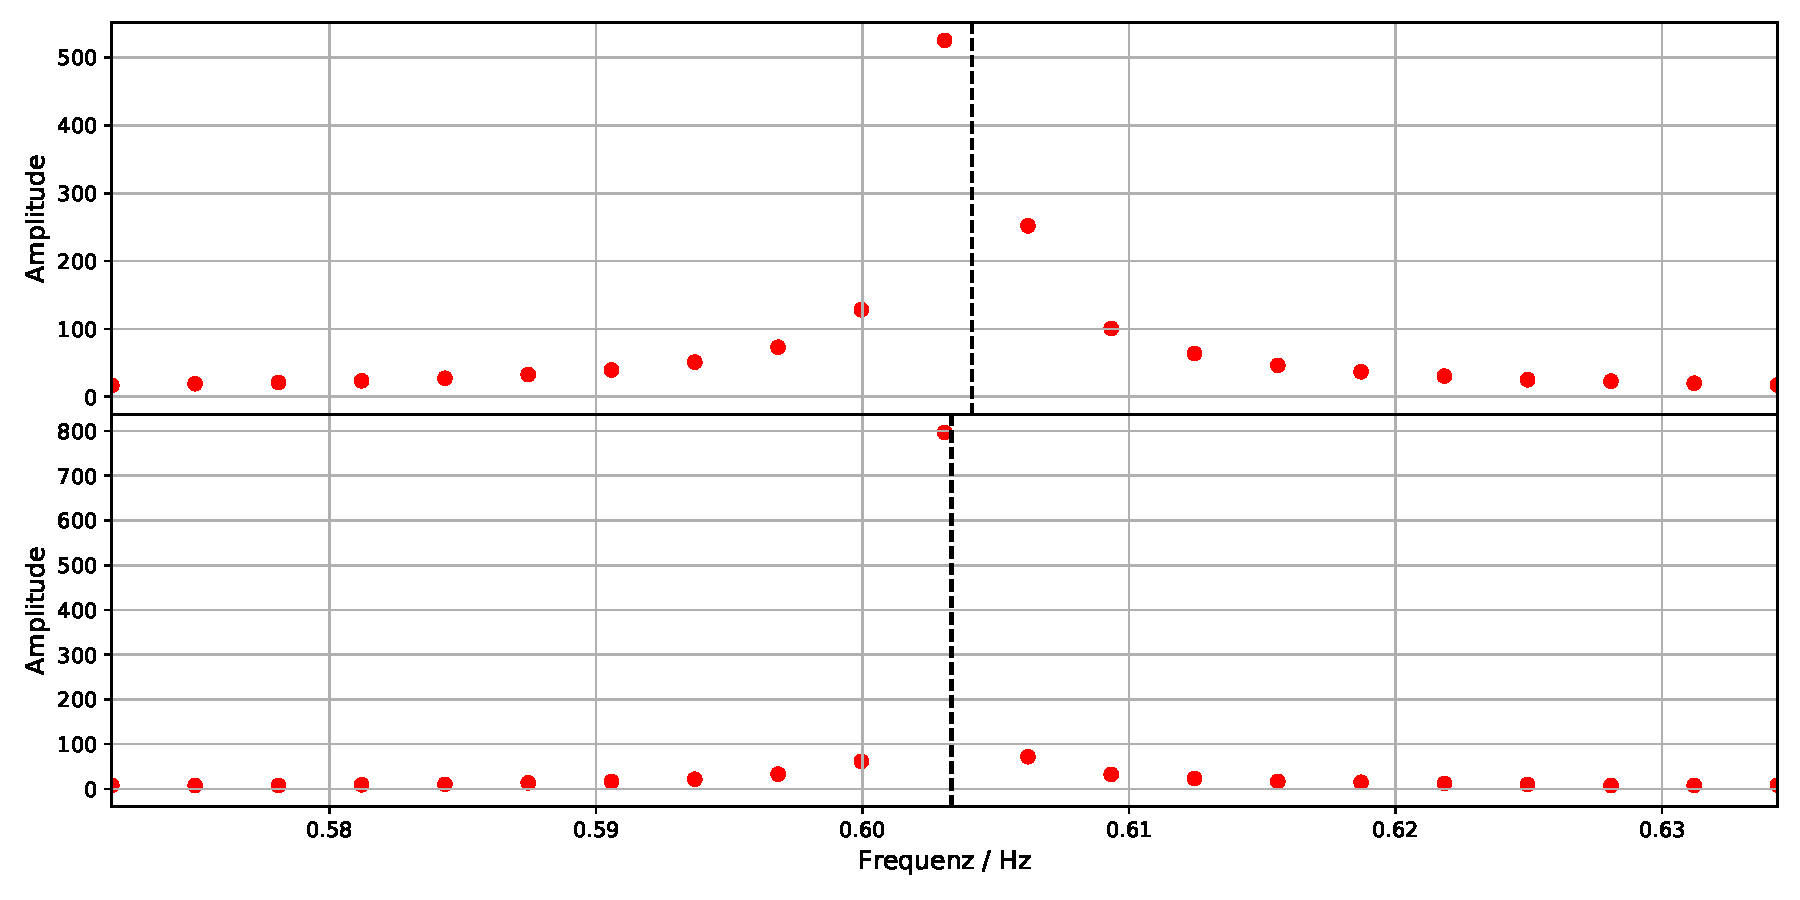
\includegraphics[width = \textwidth]{plots/fft.pdf}
	\caption{FFT der Rohdaten und Peakanalyse - oben mit Pendelkörper und unten ohne Pendelkörper}\label{plot:fft}
\end{figure}

Eine Analyse der Schwingung mit Hilfe einer FFT liefert die Ergebnisse $\omega_p = 2\pi f_p =  3.79567 \text{Hz}$ und $\omega_{st} = 2\pi f_s = 3.79093 \text{Hz}$ und passt somit zu den Werten, die die Regressionsanalyse liefert. Der Plot davon ist in Abbildung \ref{plot:fft} dargestellt. Aufgrund der mangelnden Fehleranalyse wird ausschließlich mit den Werten aus der Regressionsanalyse weitergearbeitet. \\
Aus den bisher bestimmten Größen ergibt sich eine Erdbeschleunigung von 
$$ g = \omega_p^2l_p \left( 1 + \frac 12 \frac{r_p^2}{l_p^2} \right) = 9.8184 \frac{\text{m}}{\text{s}^2}\text{.}$$
Um die Fehlerbetrachtung durchzuführen, wird $g$ als Funktion in $\omega_p$, $l_p$ und $r_p$ betrachtet. Wie in der Praktikumsanleitung für den Versuch diskutiert, kann der Fehler in $r_p$ vernachlässigt werden. Die relative Abweichung von Schwingung mit und ohne Pendelkörper beträgt
$$\frac{\lvert \omega_p - \omega_{st}\rvert}{\omega_p} = 0.0014$$
und wird daher ebenfalls vernachlässigt. Für die relevanten partiellen Ableitungen von $g$ gilt
$$\frac{\partial g}{\partial \omega_p} = 2\omega_p l_p \left(1+\frac 12 \frac{r_p^2}{l_p^2}\right) \text{ und}$$
$$\frac{\partial g}{\partial l_p} = \omega_p^2 \left(1-\frac 12 \frac{r_p^2}{l_p^2}\right)\text{.}$$
Das ergibt einen Fehler von
$$\sigma_g = 0.010 \frac{m}{s^2}\text{.}$$

\subsection{Fazit}
Die Physikalisch-Technische Bundesanstalt gibt in einer ihrer Publikationen\footnote{\url{https://www.ptb.de/cms/fileadmin/internet/fachabteilungen/abteilung_1/1.1_masse/1.15/gravzonen.pdf}} die Erdbeschleunigung für die Stadt Brüssel mit $g = 9.811 \frac{\text{m}}{\text{s}^2}$ an. Da Aachen und Brüssel näherungsweise den gleichen Breitengrad haben (Brüssel: 50.84°, Aachen: 50.78°), wird dieser Wert als Literaturwert verwendet. \\
Der Literaturwert liegt im $1\sigma$-Intervall des im Experiment bestimmten Wert $9.818 \frac{\text{m}}{\text{s}^2} \pm 0.010 \frac{\text{m}}{\text{s}^2}$ und somit innerhalb der Fehlertoleranz. Der schwerwiegendste Fehler im Experiment wurde durch die Messung der Länge $l_0$ gemacht. 